\documentclass[a4paper]{article}

\usepackage[english]{babel}
\usepackage[utf8]{inputenc}
\usepackage{amsmath}
\usepackage{caption}
\usepackage{siunitx}
\usepackage{graphicx}
\usepackage{textcomp}
\usepackage{gensymb}
\graphicspath{{./}}
\usepackage[colorinlistoftodos]{todonotes}
\usepackage[section]{placeins}
\setlength{\parindent}{0pt}
\usepackage{url}
\usepackage{bm}
\usepackage{wasysym}
\usepackage{csquotes}

% Extra units
\DeclareSIUnit\parsec{pc}
\DeclareSIUnit\megaparsec{Mpc}
\DeclareSIUnit\lightyear{ly}
\DeclareSIUnit\erg{erg}
\DeclareSIUnit\year{y}
\DeclareSIUnit\solarmass{M_{\astrosun}}
% End

\title{Lecture Notes Observational Astronomy}
\author{Mick Veldhuis}
\date{\today}

\begin{document}
\maketitle

\begin{abstract}
    Note for chapter 2 and 3, chapter 1 of the book An ``Introduction to Modern Astrophysics'' might give a bit more insight.
\end{abstract}

\tableofcontents

\section{Part 1: Photons}

\subsection{Photons}
The energy of a photon is given by $E=h\nu$, and if a photon is emitted from a blackbody then the average energy is given as $E_{avg}\approx k_BT$. Therefore $h\nu\approx k_BT$. And remember that the peak wavelength is given by $\lambda_m T=0.29 \ \si{\centi\meter\kelvin}$. As such it is important to note that the average wavelength does not equal the peak wavelength.

\subsection{Important EM Bands}
These are the main EM bands from large to smaller wavelengths and from where they are mainly / best measured.
\begin{enumerate}
    \item Radio (Ground)
    \item Millimeter (Ground)
    \item Submillimeter (Ground)
    \item IR 
    \begin{enumerate}
        \item Near-IR (Ground)
        \item Mid-IR (Space)
        \item Far-IR (Space)
    \end{enumerate}
    \item Optical (Ground)
    \item Visible (Ground)
    \item UV 
    \begin{enumerate}    
        \item Near-UV (Space)
        \item Far-UV (Space)
        \item Extreme-UV (Space)
    \end{enumerate}
    \item X-ray (Space)
    \item Gamma-ray (Space)
\end{enumerate}

\subsection{Flux density}
The spectral flux density is the energy per time per area per frequency and denoted by $S(\nu)$. But the energy received by a telescope would be $P=S_{avg}(\nu)A_{eff}\Delta\nu$, where $S_{avg}(\nu)$ is the the flux density averaged over the full bandwidth. As the average flux density and effective area are mostly not constant:

\begin{equation}
    P=\int_{\nu_1}^{\nu_2}S(\nu)A_{eff}d\nu
\end{equation}

We can then define the flux density ($F$) as the total power flowing across an area:

\begin{equation}
    F=\int_{\nu_1}^{\nu_2}S(\nu)d\nu
\end{equation}

We have another property called the luminosity $L=4\pi r^2F$, which is measured over a specific piece of the EM band $\Delta\nu$. If $\Delta\nu$ contains all frequencies then we call it the bolometric luminosity.

\bigskip

We can also define the photon spectral flux density $S_{\gamma}(\nu)$ as NUV-optical-NIR detectors measure magnitudes by the amount of photons collected in a given time. Thus we obtain

\begin{equation}
    S_{\gamma}(\nu)=\frac{S(\nu)}{h\nu}
\end{equation}

Then the number of photons per unit time and unit area detected is the photon spectral flux density times an efficiency factor $\epsilon(\nu)$:

\begin{equation}
    F_\gamma=\int_{0}^{\infty}S(\nu)\epsilon(\nu)\,d\nu
\end{equation}

This $\epsilon(\nu)$ includes all effects like the filter curve, deterctor efficiency, absorption and scattering of the telescope, instrument, and atmosphere, etc.

\subsection{Magnitudes}

They are defined as follows, if we consider two stars with fluxes $F_{\gamma, 1}$ and $F_{\gamma, 2}$,

\begin{equation}
    m_2-m_1=-2.5\log\bigg(\frac{F_{\gamma, 2}}{F_{\gamma, 1}}\bigg)
\end{equation}

This defines the apparent magnitude as seen by the detector. So if a star 2 is 100 times brighter than star 1, it is 5 magnitudes brighter, meaning 5 magnitudes less. We can summarize some useful facts (1)

\begin{equation}
    m_1-m_2\approx 0.921\ln(f_1/f_2)
\end{equation}

(2) if $\Delta f<< 1$, then $\Delta m=m_2-m_1\approx 1.086\Delta f$. (3) A factor of 2 difference in brightness is a difference of 0.75 magnitudes.

\bigskip

Now we can look back at $\epsilon(\nu)$, which is written as $\epsilon(\nu)=f_{\nu}R_{\nu}T_{\nu}$, here $f_{\nu}$ is the transmission of any filter used to isolate the region of interest. $R_{\nu}$ is the transmission of the telescope, optics, and detector. $T_{\nu}$ is the transmission of the atmosphere, if applicable. We can easily vary $f_\nu$, for instance we can measure using a $B$ filter.

\bigskip

We can now define the color of an object as the magnitude difference of the object in two different bandpasses. For instance if the filters are $X$ and $Y$, then the color $(X-Y)$ is given as

\begin{equation}
    (X-Y)\equiv m_X-m_Y=-2.5\log\bigg(\frac{F_{\gamma, X}}{F_{\gamma, Y}}\bigg)
\end{equation}

A well known magnitude system is the \textbf{Vega system}, it defines a set of A0V stars as having $m=0$ in all bands. The \textbf{Johnson-Cousins-Glass system} is a Vega system where the magnitudes of all bands in the system are set to 0 for an idealized A0V star at $\approx 8 \ \si{\parsec}$. Another common one is the \textbf{AB system} in which magnitudes are defined as

\begin{equation}
    m_{AB, \nu}=-2.5\log\big[S(\nu)\big]-48.60
\end{equation}

We shall also define the \textbf{absolute magnitude} $M$, we set the distance of the star at 10 \si{\parsec}, such that

\begin{equation}
    \mu=m-M=-2.5\log\bigg[\frac{F_{\gamma}(r)}{F_{\gamma}(10 \ \si{\parsec})}\bigg]=5\log r(\si{\parsec})-5
\end{equation}

And we define the \textbf{absolute bolometric magnitude} as the total power emitted over all frequencies expressed in magnitudes, we set the zeropoint to that of the sun $M_{bol, \astrosun}=4.74$, so that

\begin{equation}
    M_{bol}=-.5\log\bigg(\frac{L}{L_{\astrosun}}\bigg)+4.74
\end{equation}

for $L_{\astrosun}=3.845\cdot 10^{33}\ \si{\erg\per\second}$.

\section{Part 2: Positional Astronomy}

\subsection{Coordinate system}

Before we dive in we need the concept of the \textbf{Celestial sphere}, an assumption that all astronomical sources are infinitely far away and live on the surface of a sphere at infinite distance. The motion on this sphere, thus normal to the line of sight, is called proper motion. We also need the \textbf{great circle}, a circle on the surface of a sphere intercepting a plane that intersects the origin of the sphere. Which is a circle on the surface of a sphere that divides that sphere into two equal hemispheres. 

\subsubsection*{Horizontal (Alt-Az) coordinates}

\begin{figure}[ht]
\centering
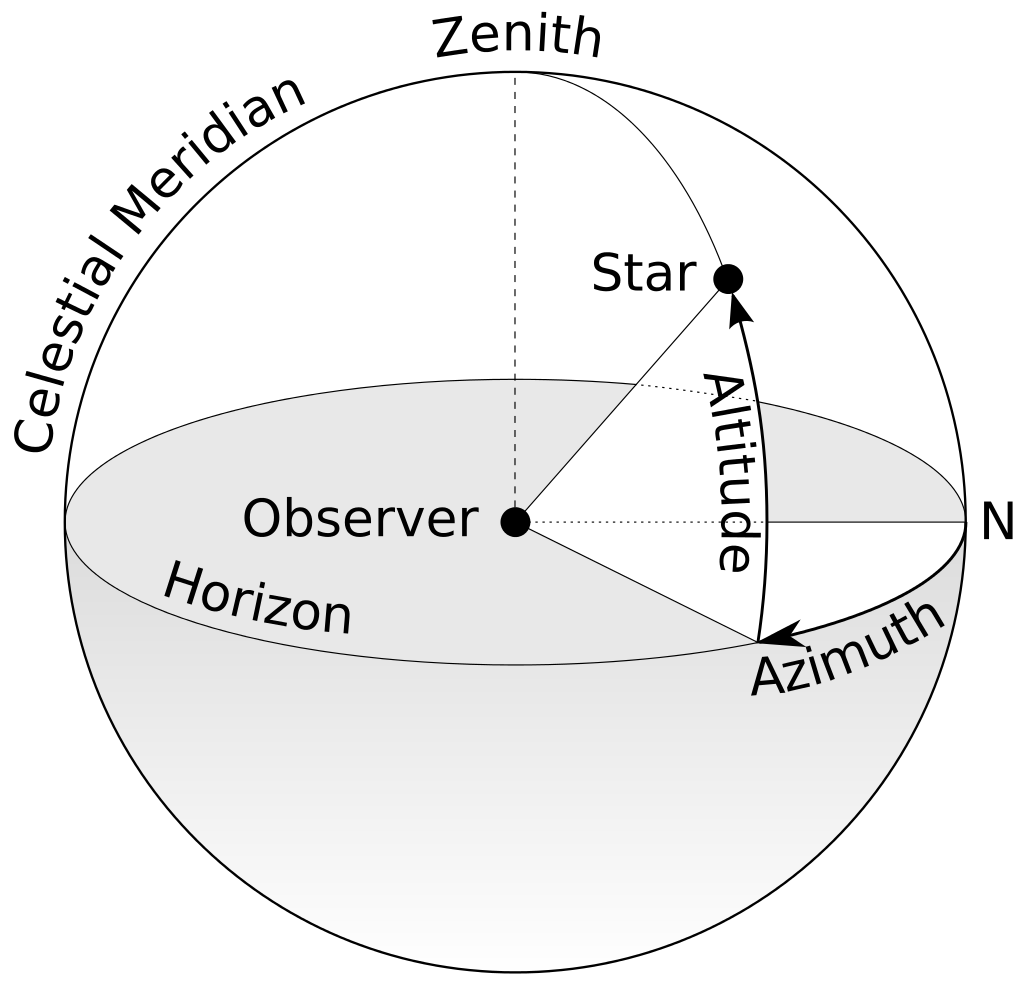
\includegraphics[width=4cm]{img/horizontal.png} \\
\caption*{\textbf{Figure 1}: The Horizontal Coordinate System.}
\end{figure}

In this system (depicted in figure 1) the great circle of the horizon projected on the celestial sphere is the equator of this system. We have two coordinates: The \textbf{altitude} (or elevation), and the zenith is at $+90\si{\degree}$. And the \textbf{azimuth}, which is measured from the north (at $0\si{\degree}$) towards the east. We also define the \textbf{meridian}, a line of constant longitude (at constant $+90\si{\degree}$). The origin is defined as the observer, and the coordinate system is left-handed.

\subsubsection*{Equatorial coordinates}

In this system (depicted in figure 2) the celestial equator is the great circle that intersects both the celestial sphere and the Earth's equator. We define the \textbf{declination} $\delta$ as the celestial latitude, with $0\si{\degree}$ at the equator, and positive towards the north. The \textbf{right ascension} (RA) $\alpha$ is the celestial longitude, measured in time (0-24 hours) from west to east, we define $0^h$ at the sun's position when it crosses the equator from south to north (noon on 21 March in Greenwich). When $\alpha=0^h$ and $\delta=0\si{\degree}$ we call the position the \textbf{vernal equinox} (\vernal). This is a right-handed system. We also have the \textbf{ecliptic}, the plane of Earth's orbit around the sun.

\bigskip 

Note that because the Earth precesses the vernal equinox and the celestial equator move w.r.t. the background objects. So we need to assign an epoch (a date) to any equatorial coordinate. Two common epochs are:

\begin{enumerate}
    \item \textbf{B1950}: Based on the Besselian year, and refers to the Earth's orientation at $22^h\,09^m$ UT on 1949 December 31. It is based on the Fundamental Katalog 4 (FK4).
    \item \textbf{J2000}: Based on the Julian year and refers to the Earth's orientation at noon in Greenwich on 2000 january 1. It is based on the ICRS, the International Celestial Reference System.
\end{enumerate}

\begin{figure}[ht]
\centering
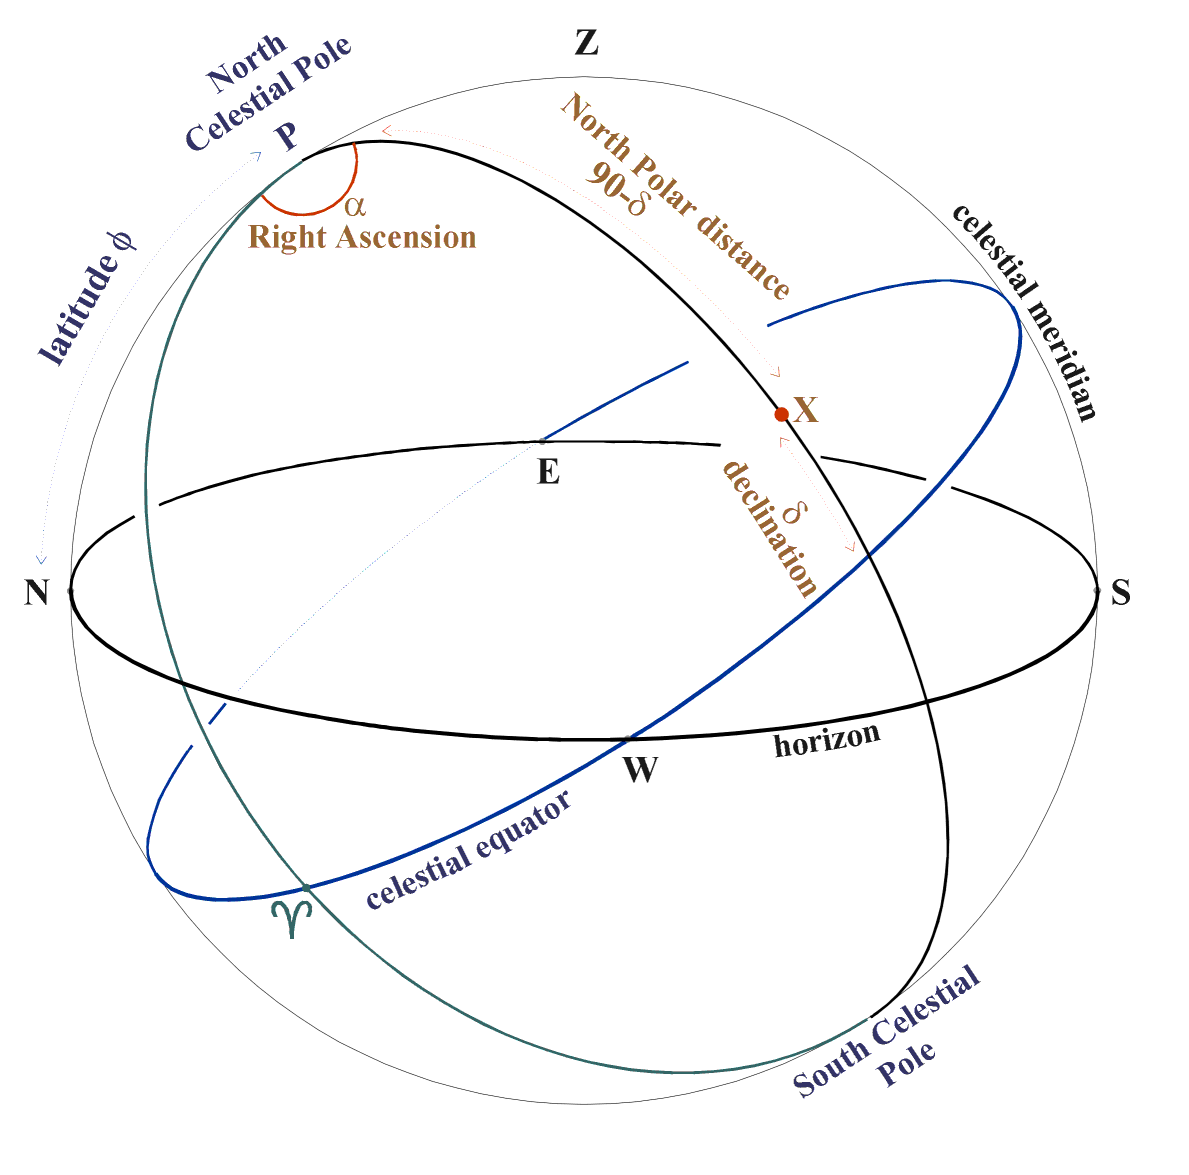
\includegraphics[width=8cm]{img/equatorial.png} \\
\caption*{\textbf{Figure 2}: The Equatorial Coordinate System.}
\end{figure}


There's also the \textbf{local equatorial system}, that is used to point polar-axis telescopes. They rotate around an axis parallel to the Earth's axis of rotation. Thus the field of the image does not rotate, as with alt-az telescopes. Here the RA is replaced by the \textbf{hour angle} (HA), HA=LST-RA, LST is the \textbf{local sidereal time}. HA varies from -6 h at the eastern horizon (rising) to 0 h at the zenith to +6 h at the western horizon (setting). This system is left-handed.

\bigskip

A general note for equatorial type coordinates: Fined angular sizes get longer in longitude (RA) as one goes towards the pole by a factor that goes as $1/\cos\delta$.

\subsubsection*{Galactic coordinates}

\begin{figure}[ht]
\centering
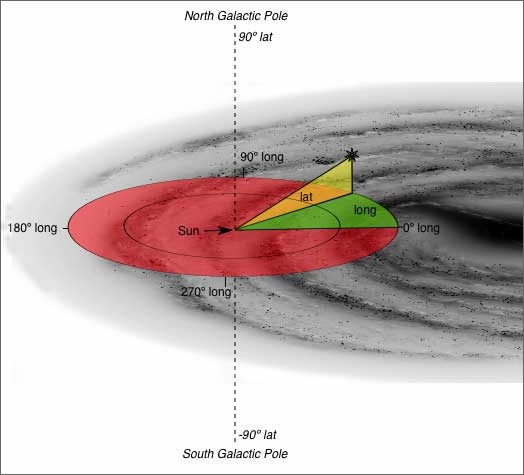
\includegraphics[width=6cm]{img/galactic.jpg} \\
\caption*{\textbf{Figure 3}: The Galactic Coordinate System.}
\end{figure}

Now the plane of the galaxy defines the equator. We have two coordinates: The \textbf{galactic longitude} $l$, measured in degrees where $0\si{\degree}$ is the line of sight with the center of the galaxy, it increases in a right-hand fashion. And \textbf{galactic latitude} $b$, with $0\si{\degree}$ at the equator.

\bigskip

The system is precisely defined by the NGP, which sits at $\alpha_{NGP}=192.25\si{\degree}=12^h\,49^m$ and $\delta_{NGP}=+27.4\si{\degree}=+27.4\si{\degree}\,24'$. And by the galactic longitude of the celestial pole $l_{NCP}=123\si{\degree}$. Thus the celestial and galactic equator are tilted by $90\si{\degree}-27.4\si{\degree}=62.6\si{\degree}$.

\bigskip 

Note that the galactic system is specified in B1950.


\subsubsection*{Other coordinate systems}

We have two others that are of interest, \textbf{Ecliptic coordinates} and \textbf{Supergalactic coordinates}. The former uses the plane of the ecliptic as the celestial equator and is mostly used for satellite navigation. The latter is used for determining the positions of galaxies and clusters relative to the Virgo Cluster-Local Group-Coma Cluster plane.

\subsection{Motions of stars}

We assume the horizontal coordinate system for now. And consider Groningen (at $\theta_{lat}\approx+53\si{\degree}$). 

\bigskip

Stars with a declination $\delta=(\theta_{lat}-90\si{\degree}, 90\si{\degree}-\theta_{lat})$ rise from the east and set in the west, stars with $\delta>90\si{\degree}-\theta_{lat}$ circle around the NCP, and are always above the horizon. Stars with $\delta=(0, 90\si{\degree}-\theta_{lat})$ rise north of east, moves towards the south until they transit the meridian, then move westwards and set north of west. They cross the meridian at a maximum altitude $\theta_B=90\si{\degree}-\theta_{lat}+\delta$.

\bigskip

Let us quickly define the \textbf{parallax}, the Earth is at a distance 1 AU from the sun, six months later, the earth is at a position opposite in orbit. But the observed star has remained in the same place relative to the sun. Then from Earth the star has subtended an angle $2\varpi$ on the sky. If $r=1$ AU, we find that 

\begin{equation}
    \frac{r}{d}=\tan\varpi\approx \varpi \ \text{rad}
\end{equation}

we can easily convert $\varpi$ to arc seconds as $\varpi ''=206265\,\varpi \ \text{rad}$, so that 1 AU is as $d=206265\ \text{AU}/\varpi''$. We note that 1 \si{\parsec} is the distance at which a star has a parallax of $\varpi=1''$. And the distance to a star with parallax $\varpi$:

\begin{equation}
    d=\frac{1}{\varpi''}\si{\parsec}
\end{equation}

If the star lies at the ecliptic pole, it traces out a circle on its parallactic path; and if the star lies in the ecliptic plane, it traces out a line.

\subsubsection*{Aberrations}

The velocity of the Earth in the orbit with the sun causes an apparent shift of stellar positions, it's an effect of special relativity, these effects are called \textbf{aberrations}. It is similar to how rain appears to fall in different situations e.g. standing still or in a (moving) train. The maximum effect is a few arc seconds as per

\begin{equation}
    \theta_{aber, max} \approx \frac{v_{Earth}}{c}\approx \frac{10^6\ \si{\centi\meter\per\second}}{10^{10}\ \si{\centi\meter\per\second}}=20.5''
\end{equation}

for objects perpendicular to the Earth's orbit (the ecliptic). So a star at the ecliptic pole will trace at a circle of 20.5'' every year. This effect depends entirely on the time of year and the direction of the object. The Earth's rotation also causes aberrations, diurnal aberrations (effects of $\theta<0.3''$).

\subsubsection*{Precession and nutation}

\textbf{Precession} of the Earth's axis w.r.t. the ecliptic, caused by torques from nearby planets (very little), the sun, and our moon, causes the equatorial system to precess w.r.t. the background stars. Due to Earth not being spherical, other objects can exert a torque on it. A full precessional period is 25770 years. As a result the celestial equator moves as well. Therefore the vernal equinox also changes (it is called \textbf{precession of the equinoxes}) and it is the reason we should always specify a date in the equatorial system, this precession is $50.3\si{\arcsecond\per\year}$

\bigskip

We also have \textbf{nutation}, the small scale wobbles around the steady precession, which is caused by the same processes, plus some less-predictable wobbles due to ocean-crust interactions on earth. The effect is $<1\si{\arcsecond\per\year}$.

\bigskip 

On top of these two effects we should also not forget the proper motion of stars and atmospheric refraction.

\section{Time}

\subsection{The calendar and seasons}

The vernal equinox is always the time at which the sun crosses from the southern to the northern hemisphere on the celestial sphere. Thus the seasons are indicated by the right ascension of the sun. 

\bigskip

We define a \textbf{sidereal year} as the time it takes for the sun complete a full circuit of the background stars and return to its original position, such that one year is approximately 365.26 days.

\bigskip

What we know as the \textbf{Julian calendar} is tied to the seasons, so that 21 March should always take place at the beginning of spring, even though the $\vernal$  keeps moving w.r.t. the background stars. So this calendar is based on the \textbf{tropical year} and it has exactly 365.25 days, the time between successive \vernal s, this year is approximately 365.24 days. We now come to Pope Gregory XIII, who reset the vernal equinox and removed the leap days from century years not evenly divisible by 400 (e.g., 1700 or 1800). This means that the \textbf{Gregorian calendar} is now (as good as) synchronous with the tropical year. 

\subsection{Different \textit{times}}

\subsubsection*{Sidereal time}

The \textbf{local sidereal time} is the RA of the meridian passing directly overhead, i.e. the RA of the zenith right now.

\subsubsection*{Solar time}

The \textbf{solar time} is defined by the transit of the sun through the meridian, meaning the sun is at the highest point in the sky at noon solar time. It clearly has a variable length due to the eccentricity of the Earth's orbit around the sun and the tilt of the Earth's axis w.r.t. the ecliptic (the so called \textbf{obliquity}), near the equinoxes the ecliptic's projection onto the celestial equator is smaller than near the solstices. Due to this variation ($\approx\pm 15 \si{\minute}$ throughout the year), we define the \textbf{mean solar time} that sets the day length to a constant 24 hours. An interesting phenomenon is the so called \textbf{analemma}, it is a diagram showing the position of the sun in the sky, as seen from a fixed location on Earth at the same mean solar time, such that the position varies over the course of a year. 

\bigskip

Sort of a problem arises, since the MST depends on the position of the observer. To deal with this issue time zones were introduced, with the zeropoint at $0\si{\degree}$ longitude (at Greenwich), this position is called the prime meridian. Due to the sun moving along the ecliptic $\approx 1\si{\degree\per\day}$, the Earth has to rotate one degree extra every day to keep up with the sun. As such a solar day is $\approx 4\si{\minute}$ longer than a sidereal day, so 1 mean solar day $= 24^h\,00^m\,00^s$ and 1 sidereal day $= 23^h\,56^m\,04.09^s$

\subsubsection*{Universal time (UT1)}

\textbf{Universal time} (UT1) is based on the motion of the fixed stars, but is adjusted such that it is approximately equal to the mean solar time at Greenwich. Formally, $00^h\,00^m\,00^s$ (midnight in Greenwich) on 1 January is defined to occur at Greenwich LST $\approx 6.7^h$.

\subsubsection*{Physical time}

\textbf{Physical times} are based on physical measurements, the second for instance is based on the hyperfine transition of 133-Cesium

\bigskip

For example the atomic time \textbf{TAI}, is based on ~150 atomic clocks on tens of countries. We also have \textbf{Terrestrial time} (TT), which is not adjusted for variations in the Earth's rotation, it is based on ephemeris time (ET), it has exactly 86400 seconds in a year. It's exact definition would be TT = TAI + 32.184 s to match ET. There also are relativistic timescales, they try to synchronize times across the Solar System.

\subsubsection*{Universal time (UTC)}

To link the TAI and UT1 systems, \textbf{Universal coordinated time} (UTC) was fabricated. It is actually based on TAI, but it includes a leap second to keep within a 0.9 seconds of UT1. Such that some years contain 86400 $\pm$ 1 seconds.

\subsection{Julian dates}

The \textbf{Julian date} (JD) is defined as the number of Julian days since noon on 1 January 4713 BCE, roughly 24/04/2019 at $1^h\,00^m\,00^s$ UT1 is JD 2458598.0. So the beginning of each day is defined as $12^h$ UT1 in Greenwich. Often the \textbf{modified Julian date} (MJD) is used, MJD = JD - 2400000.5, this starts at midnight instead of noon. The J2000 system is defined by the Julian days/years and began at $12^h$ 01/01/2000 (JD 2451545.0)

\section{Telescopes and optics}

What do we actually measure with our telescopes (+ instrument + detector): the rate of arriving photons, the arrival direction (says something about position and shape), the photon energy (to determine the spectrum), and the polarization of the EM wave. In the end we wish to maximize its sensitivity (the signal to noise ratio).

\subsection{Telescope types}

\subsubsection*{Refractors}

These \textbf{refractors} are two-lens telescopes, they are limited by the size of the lenses ($\le 1\ \si{\meter}$).

\subsubsection*{Reflectors}

These \textbf{reflectors} use mirrors instead of lenses, there exist various n-mirror configurations. One-mirror telescopes have a single mirror that directs the light to a detector at the prime focus, a prime focus corrector is needed to eliminate aberrations. There are then also various two-mirror systems, the \textbf{Newtonian} is very common. It uses a concave mirror to direct the light to a flat mirror that bends it from the prime focus to, e.g., a detector. Other two-mirror telescopes are the \textbf{Cassegrain}, it has a convex secondary mirror; and the \textbf{Gregorian}, with a concave secondary. The most common configuration for three-mirror telescopes is the \textbf{Nasmyth} configuration, it looks like a Cassegrain or Gregorian with a fold mirror to send the beam onto a platform attached to the azimuth drive of an alt-az telescope, handy for large instruments requiring long focal lengths (slow $f$-ratios) and mechanical stability.

\subsection{Gaussian optics}

As seen in the image above, where refraction is covered, reflection is just a special case for which $n'=-n$. For the remaining part of this section we assume that the point P is close to the optical axis and that the angles are small such that the \textbf{paraxial approximation} holds, meaning that $\sin\theta\approx\theta$ and $\tan\theta\approx\theta$ for any $\theta$. We can then write \textbf{Snell's law} of refraction as  

\begin{equation}
    n\sin i = n'\sin i'\quad\Rightarrow\quad ni = n'i' 
\end{equation}

where the right-hand is the law in the paraxial approximation. With our approximation we assume that $\phi=y/R$, $u=y/s$, and $u'=y/s'$. Such that we can obtain

\begin{equation}
    \frac{n'}{s'}-\frac{n}{s}=\frac{n'-n}{R}
\end{equation}

Now, if either $s$ or $s'=\infty$, then the conjugate's distance is called the \textbf{focal length} (denoted by $f'$ or $f$). So if $s'=\infty\Rightarrow s=f$ and if $s=\infty\Rightarrow s'=f'$. We define the \textbf{power} ($P$) of a surface as $(n'-n)/R$, the power does not depend on the direction. So we obtain the Gaussian equation for a single refracting surface:

\begin{equation}
    \frac{n'}{s'}-\frac{n}{s}=P=\frac{n'}{f'}=\frac{n}{f}
\end{equation}

This equation does not depend on, the height of the point P, $y$. Therefore the equation also applies to object and image points close, but not on, the optical axis. Such as the next figure, where if $\phi$ is small BQ and B'Q' are perpendicular to the line segment BCB'. Such that we determine the \textbf{tranverse magnification} ($m$), the ratio of image height to object height $m=h'/h$ for $h'=-\phi(s'-R)$ and $h=-\phi(s-R)$, note that $h$ and $h'$ have opposite signs. We obtain

\begin{equation}
    m=\frac{h'}{h}=\frac{s'-R}{s-R}=\frac{ns'}{n's}
\end{equation}

In the previous figure $m$ is obviously negative, as the image is inverted. We then define the \textbf{angular magnification} ($M=\tan u'/\tan u$), for $y=s\tan u=s'\tan u'$, therefore 

\begin{equation}
    M=\frac{\tan u'}{\tan u}=\frac{s}{s'}=\frac{n}{n'm}=\frac{nh}{n'h'}
\end{equation}

This equation relates the transverse and angular magnification for a pair of conjugate planes, i.e. the sky and the detector. Which can be rewritten as

\begin{equation}
    nh\tan u=n'h'\tan u'\quad\Rightarrow\quad nhu=n'h'u'
\end{equation}

Let $H=nh\tan u$, then $H$ is invariant in an optical system. As such the total flux collected by an optical system is proportional to $H^2$. Now let's find the paraxial equation for reflection, where $i=-i'$, such that $i'$ is positive. We then obtain the \textbf{reflection law}:

\begin{equation}
    \frac{1}{s}+\frac{1}{s'}=\frac{2}{R}
\end{equation}

Which could also be obtained via earlier results and $n'=-n$. We also obtain 

\begin{equation}
    \frac{1}{s}+\frac{1}{s'}=\frac{2}{R}=-\frac{P}{n}=\frac{1}{f'}=\frac{1}{f}
\end{equation}

which tells us that a concave mirror has $P>0$ versus convex one with $P<0$, and

\begin{equation}
    m=-\frac{s'}{s}
\end{equation}

We often take $f>0$ for a concave mirror and $f<0$ for convex ones, although this is not very valid. For a two-surface system we find the net power to be

\begin{equation}
    P=P_1+P_2-\frac{d}{n}P_1P_2
\end{equation}

where $n>0$ and $d>0$. For a thin lens we obtain

\begin{equation}
    \frac{1}{s'}-\frac{1}{s}=(n-1)\bigg(\frac{1}{R_1}-\frac{1}{R_2}\bigg)=P_1+P_2=P=\frac{1}{f'}=\frac{1}{f}
\end{equation}

As such the net power of a thin lens is the reciprocal of its focal length, which is the same as a thick lens with $d=0$. Lastly, consider a thick plane-parallel plate in air. This plate has no optical power, but it shifts the image along the optical axis by a distance $\Delta$ relative to the object:

\begin{equation}
    \Delta = s_2'-s_1+d=d\bigg(1-\frac{1}{n}\bigg)
\end{equation}

where $d$ is the distance between the parallel-plates. When we look at actual telescopes we shall encounter the \textbf{focal ratio} $F_1=f_1/D$, where $D$ is the telescope diameter. $F=f/D$ is the final focal ratio, and $f$ is the effective focal length. We then find the net power to be

\begin{equation}
    P=P_1\bigg[1-\bigg(\frac{k}{\rho}\bigg)\bigg]=\frac{P_1}{m}
\end{equation}

where $k$ is the ratio of the marginal rays of the secondary and primary mirrors (radii of the mirrors), and $\rho$ is the ratio of the vertex radii of curvature. Note that the power is positive for a Cassegrain telescope and negative for a Gregorian telescope. And in terms of focal lengths and focal ratios we have

\begin{equation}
    m=\frac{f}{f_1}=\frac{F}{F_1}
\end{equation}

From which we can conclude that a Gregorian requires a bigger secondary to cover the same angular diameter field. 

\subsection{Telescope plate scales and speeds}

The \textbf{plate scale} ($S$) is the angle imaged onto a unit length on the focal plane, such that $S=\theta/h'=1/f$, or conveniently

\begin{equation}
    S (\si{\arcsecond\per\milli\meter}) = \frac{206265 \ [\si{\arcsecond\per\radian}]}{f \ [\si{\milli\meter}]}
\end{equation}

The term $f$-ratio ($f/F$) is often thrown around. We have that the speed of an optical system is proportional to the energy deposited in a unit area (such as a pixel), so $v\propto E_{pixel}\propto F^{-2}$. The speed of an optical system only depends on the focal ratio (which characterizes how quickly a bundle of rays converges as the rays form an image) and is independent of the diameter. Fast systems are prone to aberrations due to the large range of angles incident on the focal point or plane, so they are difficult to focus. And they are essential for wide-field imaging or broadband spectroscopy. On the other hand slow optical systems are needed to produce fine plate scales, for more detail.

\subsection{Optics via Fermat's principle}

Let's first define \textbf{Fermat's principle}, it basically says that the travel time of a ray is infinitesimally close to that of a neighboring path. So given a surface between two points $P_0$ and $P_1$ (in the $yz$-plane), for a travel time $\tau$:

\begin{equation}
    \frac{d\tau}{dy}=\frac{d\tau}{dz}=0
\end{equation}

In optics we shall use the words \textbf{optical path length} (OPL) instead of travel time ($\tau$). Which is defined as

\begin{equation}
    d(\text{OPL})=c\,dt=\bigg(\frac{c}{v}\bigg)v\,dt=n\,ds
\end{equation}

for $ds$ is the infinitesimal path length. Such that

\begin{equation}
     c\int\,dt=\int n(y, z)\,ds=\int n(y, z)\sqrt{((dy)^2+(dz)^2)}
\end{equation}

Note that the index of refraction can depend on the position. We now apply the caclulus of variations, to the integral, to obtain the following equation:

\begin{equation}
    \frac{\partial F}{\partial y}-\frac{d}{dz}\bigg(\frac{\partial F}{\partial y'}\bigg)=0 
\end{equation}

The so-called \textbf{Euler-Lagrange Equation}, where $F=F(y, y', z)$ ($y'=dy/dz$). Which we can solve by using that $F(y, y', z)=n(y,z)\sqrt{1+y'^2}$. From which we obtain

\begin{equation}
    \frac{dn}{dz}=\frac{\partial n}{\partial z}+y'\frac{\partial n}{\partial y}
\end{equation}

Continuing $\alpha$ will be the angle made by the tangent of the path with the $z$-axis. Note that the path the ray takes has a curvature $K$:

\begin{equation}
    K=\frac{d\alpha}{ds}=\cos\alpha\frac{d\alpha}{dz}
\end{equation}

such that (we obtain his important result!)

\begin{equation}
    nK=n\cos\alpha\frac{d\alpha}{dz}=\cos\alpha\frac{\partial n}{\partial y}-\sin\alpha\frac{\partial n}{\partial z}
\end{equation}

This is the equation for the local curvature of a light ray subject to Fermat's principle in a medium in which $n=n(y,z)$. If we let $n=cst$, then $K=0$ such that the ray travels in a straight path. Let's cover a few applications / examples.

\subsection{Atmospheric refraction}

First, assume that the atmosphere is a flat layered medium with $n=n(z)$, where $z$ points towards the center of the Earth, such that the curvature of the Earth is negligible. We then have

\begin{equation}
    nK=n\cos\alpha\frac{d\alpha}{dz}=-\sin\alpha\frac{\partial n}{\partial z}
\end{equation}

As the change in $n$ is rather small, the path ray from a star will not be significantly deviated if $\alpha$ is not close to $90\ \si{\degree}$. We can then integrate the previous expression to find

\begin{equation}
    \delta\alpha=-\tan\alpha_0\,\delta n
\end{equation}

here $\alpha_0$ is the zenith angle at the top of the atmosphere. Now, for a ray passing down through the atmosphere $\delta n>0$ and $\delta\alpha < 0$, such that the ray is bend towards the $z$-axis. But, note that $n$ also depends on the wavelength, so different wavelengths get bent by different amounts.

\subsection{A dispersing prism}

For which $n=n(\lambda)$ and in air $n=1$. If we consider it to have a base $t$ and sides of length $L$, and that the rays follow paths parallel to the prisms base. The OPL of the bottom ray (at the base) is $nt$, the OPL of the top ray (at the prism's vertex) is $2L\cos\alpha$. By Fermat's principle we obtain

\begin{equation}
    nt=2L\cos\alpha
\end{equation}

Let's imagine that $\theta=\theta(\lambda)$ is the angle that the (top) beam's path changes w.r.t. to its original path. We can differentiate this expression w.r.t. the wavelength, such that we in the end obtain

\begin{equation}
    \frac{d\theta}{d\lambda}=\frac{t}{a}\frac{dn}{d\lambda}
\end{equation}

where $a$ is the width of the light beam. Often $n(\lambda)=C_0+C_1/\lambda^2$ for constants $C_0$ and $C_1$. Therefore the previous equation becomes

\begin{equation}
    \frac{d\theta}{d\lambda}=-\frac{2t}{a}\frac{C_1}{\lambda^3}
\end{equation}

So $\theta$ decreases as the wavelength increases, such that blue light is deviated more than red light. Or formally, the \textbf{angular dispersion} $d\theta/d\lambda$ is larger for shorter wavelengths.

\subsection{Reflecting mirrors}

Let's consider three cases: a concave mirror with one conjugate at $\infty$, a concave mirror with both finite conjugates, and a convex mirror with both finite conjugates. 

\subsubsection*{Case I: A concave mirror with one conjugate at $\infty$}

Let $f$, $l$ (the length of the reflection from the mirror to the optical axis), and $\Delta$ be positive. Such that

\begin{equation}
    2f=l+(f-\Delta)\quad\Rightarrow\quad l=f+\Delta
\end{equation}

So that

\begin{equation}
    l^2=y^2+(f-\Delta)^2\quad\Rightarrow\quad y^2=4f\Delta=-4fz
\end{equation}

Which is a parabola with vertex $(0,0)$. Finally $y^2=2Rz$, $R$ is the radius of curvature and $R, z<0$. In 3D $y^2\Rightarrow x^2+y^2$ 

\subsubsection*{Case II: A concave mirror with both conjugates finite}

We now find that for $2a=s+s'$ and $b^2=ss'$:

\begin{equation}
    y^2-2z\frac{b^2}{a}+z^2\frac{b^2}{a^2}=0
\end{equation}

Which is an ellipse with center $(0, a)$.

\subsubsection*{Case III: A convex mirror with both conjugates finite}

We now find that for $2a=s+s'$ and $b^2=-ss'$:

\begin{equation}
    y^2+2z\frac{b^2}{a}-z^2\frac{b^2}{a^2}=0
\end{equation}

Which is a hyperbola with center $(0,0)$.

\subsubsection*{Generalization}

These forms can be generalized, consider an ellipse with eccentricity $e=c/a$ ($-1<e<1$), where $c$ is the distance from one focus to the center of the ellipse $c^2=a^2-b^2$, such that $1-e^2=b^2/a^2$, and we get

\begin{equation}
    y^2-2Rz+(1+e^2)z^2=0
\end{equation}

which is valid for any conic section. This can be rewritten by using $K$, Schwarzschild's conic constant and $\rho^2=x^2+y^2$.

\begin{table}[ht]
    \centering
    \begin{tabular}{c|c|c}
        Conic section & $e^2$ & $K$ \\
        
        \hline
        
        Prolate ellipsoid & $e^2 < 0$ & $K > 0$\\
        Sphere & 0 & 0 \\
        Oblate ellipsoid & $0<e^2<1$ & $-1<K<0$ \\
        Paraboloid & 1 & -1 \\
        Hyperboloid & $e^2 > 1$ & $ K < -1$
    \end{tabular}
\end{table}

This suggests that the primaries for both a Cassegrain and Gregorian should be paraboloid, while the secondary for a Gregorian should be an ellipsoid and a hyperboloid for a Cassegrain.

\subsection{Resolution}

We consider a perfect optical system. Light from two objects differing by an angle $\theta$ fill the aperture $D$, and the points cannot be resolved if the OPL difference between the rays is less than approximately one wavelength. In the figure in the lecture slides this OPL difference is noted as $\Delta$, so we need $\Delta >\approx \lambda$. Such that $\theta_{min}\approx\lambda/D=1.22\lambda/D$.

\subsection{Optical aberrations}

Wikipedia defines optical aberrations as

\begin{displayquote}
    $[...]$ \textit{a property of optical systems such as lenses that causes light to be spread out over some region of space rather than focused to a point.}
\end{displayquote}

These aberrations come in two main types: chromatic aberrations (dependent on wavelength) and monochromatic aberrations (independent of wavelength).

\subsubsection*{Monochromatic aberrations}

Monochromatic aberrations come in two types: those that deteriorate the image and those that deform the image. These aberrations are inherent to an optical system, and can be corrected in multiple-element system. As Gaussian optics is based on the paraxial approximation, it will break down at large distances from the optical axis or at large angles to the optical axis. So if we expand $\sin\theta$ further

\begin{equation*}
    \sin\theta=\theta-\frac{\theta^3}{3!}+\frac{\theta^5}{5!}-\dots
\end{equation*}

The first and second terms are considered in third-order aberration theory, but also higher-order (Zernike) terms can be considered. In this third-order theory, there are five primary aberrations which scale as $y^m\theta^n$, for $m+n=3$. These are Spherical aberrations (independent on the angle $\theta$), coma, astigmatism, field curvature, and distortion (independent of the distance $y$ to the optical axis). The aberrations dependent on $\theta$ are called off-axis aberrations. 

\bigskip

Those five aberrations are as follows:

\begin{enumerate}
    \item[--] \textbf{Spherical aberrations}: they occur when rays do not come to a focus at the same point on the optical axis.
    \item[--] \textbf{Coma}: rays form an off-axis source converge at different points on the focal plane. This occurs off-axis and is asymmetric because rays from the opposite side of the optical axis land on the same side of the axis. It also appears when optical elements are misaligned.
    \item[--] \textbf{Astigmatism}: they are caused by rays in the horizontal and vertical plane coming to different foci, the best focus is then called the \textbf{circle of least confusion}.
    \item[--] \textbf{Field curvature}: there is curvature of the image plane, outside the paraxial regions. This can be corrected by adding lenses or mirrors to flatten the field.
    \item[--] \textbf{Distortion}: this is the radial change in plate scale with field angle, it deforms the image.
\end{enumerate}

\subsubsection*{Chromatic aberrations}

They are caused by rays of light with different wavelengths, coming to different foci. An example would be halos of different colors around observed objects. This aberration can be corrected by creating achromatic doublets or triplets by combining positive and negative lenses. Doublets bring lights from two wavelengths to a common focus. Triplets likewise bring light from three wavelengths to a common focus. From this we can conclude that one can generally correct $n$ primary aberrations with $n$ reasonably separated powered optical elements. 

\section{Noise}

\subsection{Probability}

Some rules of probability are

\begin{align*}
    &P(X)+P(\bar{X})=1\\
    &P(X,Y)=P(X|Y)P(Y)
\end{align*}

These probabilities depend on the relevant background information, as there is no such thing as absolute probability. Using these equations we can formulate \textbf{Bayes' theorem},

\begin{equation*}
    P(X|Y)=\frac{P(Y|X)P(X)}{P(Y)}
\end{equation*}

Where $X$ would denote the hypothesis and $Y$ the data. For $P(X)$, $P(Y|X)$, $P(X|Y)$, and $P(Y)$ are respectively the prior probability, the likelihood function, the posterior probability, and the evidence. We can also define the marginalization equation as

\begin{equation*}
    P(X)=\int_{-\infty}^{\infty}P(X,Y)dY
\end{equation*}

and the marginalization condition

\begin{equation*}
    \int_{-\infty}^{\infty}P(Y|X)dY=1
\end{equation*}

\subsection{Gaussian noise}

We have that

\begin{equation*}
    P(x_k|\mu, \sigma, I)\approx\frac{1}{\sqrt{2\pi\sigma^2}}\exp{\bigg[-\frac{(x_k-\mu)^2}{2\sigma^2}\bigg]}
\end{equation*}

Such that

\begin{equation*}
    \mu_0=\frac{1}{N}\sum_{k=1}^{N}x_k
\end{equation*}

and so

\begin{equation*}
    \mu=\mu_0\pm\frac{\sigma}{\sqrt{N}}
\end{equation*}

But if the measurements are weighted

\begin{equation*}
    \mu_0=\frac{\sum_{k=1}^{N}w_kx_k}{\sum_{k=1}^{N}w_k}\ \ , \ \ w_k=\frac{1}{\sigma^2}
\end{equation*}

So

\begin{equation*}
    \mu=\mu_0\pm\bigg(\sum_{k=1}^{N}w_k\bigg)^{-1/2}
\end{equation*}

\subsection{The Poisson distribution}

The probability of observing $N$ events (i.e. photons) is given by the pdf

\begin{equation*}
    P(N|\mu,I)=\frac{\mu^Ne^{-\mu}}{N!}
\end{equation*}

\subsection{The Gaussian distribution}

If we know both the mean and variance of the data. Then we obtain 

\begin{equation*}
    P(x|\mu, \sigma, I)=\frac{1}{\sqrt{2\pi\sigma^2}}\exp{\bigg[-\frac{(x-\mu)^2}{2\sigma^2}\bigg]}
\end{equation*}

Such that, irrespective of the magnitude of $\mu$:

\begin{equation*}
    \langle (N-\mu)^2 \rangle=\sum_{N=0}^{\infty}(N-\mu)^2P(N|\mu,I)=\mu
\end{equation*}

Therefore the standard deviation of $N$ counts is $\mu^{1/2}$

\subsection{Error propagation}

For some function $f(x, y)$ we have that the variance is given as

\begin{equation*}
    \sigma_f^2=\bigg(\frac{df}{dx}\bigg)^2\sigma_x^2+\bigg(\frac{df}{dy}\bigg)^2\sigma_y^2+\bigg(\frac{df}{dx}\bigg)\bigg(\frac{df}{dy}\bigg)\rho\sigma_x\sigma_y
\end{equation*}

where $\rho$ is the correlation between $x$ and $y$. This equation holds if the covariances are known, and $f(x, y)$ is almost linear around $x\pm dx$ and $y\pm dy$.

\subsection{Signal-to-noise ratio}

The \textbf{signal-to-noise ratio} is used to express the confidence in detecting an object in astronomy. Let's say that we detect $N$ photons, then $N\approx\langle N \rangle=\mu$ (thus also with variance $\mu\approx N$). The call the detectors on noise the read noise (RN), with variance $(\text{RN})^2$. Thus the total variance is given by $\sigma^2=N+(\text{RN})^2$, thus the standard deviation is $\sigma=\sqrt{N+(\text{RN})^2}$. But as the background also produces photons $\sigma$ should be rewritten as

\begin{equation*}
    \sigma=\sqrt{N_{\text{S}}+N_{\text{B}}+(\text{RN})^2}
\end{equation*}

Therefore the signal-to-noise ratio is given as

\begin{equation*}
    \frac{S}{N}=\frac{N_{\text{S}}}{\sigma}=\frac{N_{\text{S}}}{\sqrt{N_{\text{S}}+N_{\text{B}}+(\text{RN})^2}}
\end{equation*}

Which represents the significance of the detection of our source photons in units of the error $\sigma$. Note that counts from a CCD image are in \textbf{ADU}, 

\begin{equation*}
    \text{ADU}=\frac{N_\gamma}{G}
\end{equation*}

where $G$ is the gain (in $e^{-}$/ADU).

\section{Detectors}

\subsection{The human eye}

\subsubsection*{Elements of the eye}

The eye consists of a lens (with $f\approx 24\ \si{\milli\meter}$), which focuses the light onto the back of the eye. The iris, which is an adjusting pupil that dilates and contracts, to change the speed or focal length of the eye. The retina is the detector, consisting of light-sensitive neurons on the focal plane of the eye (the center of the retina is called the fovea). Lastly, the optic nerve is the cabling that carries the signal from the retinal neurons to the brain.

\subsubsection*{The retina and retinal cells}

The human eye can detect light from $3900$ to $7800$ \si{\angstrom}, with a \textit{readout time} of about 30 \si{\hertz} and the eye is sensitive to around 9 to 10 magnitudes.

\bigskip

Then on to the retinal cells. There are around 125 million photoreceptors over the focal surface of the eye, they sense light by charges induced by photon absorption (so the retina is a chemical detector). A peculiar thing is that light will reach the photosensitive parts of the cells after passing through the \textit{cabling}. We have two types of nerve endings:

\begin{enumerate}
    \item Rods: They form 95\% of all retinal cells, they are panchromatic (black \& white) but not frequency sensitive. The active chemical is rhodopsin, when a photon is absorbed it splits off a fragment called retinaldehyde. It requires about 1 to 10 photons to trigger a rod. Also, many rods are bundled together by a single nerve fiber. Lastly, the regeneration of rhodopsin takes about 30 minutes.
    \item Cones: They are larges than rods, form about 5\% of the retinal cells and they are color sensitive. The active chemical is iodopsin. The cones come in blue, green, and red (1:4:8).
\end{enumerate}


There are two types of vision \textbf{photopic vision}, meaning that cones do the work as in bright light the rods are not sensitive. And \textbf{Scotopic vision}, the rods are active in dim light (as are cones, but at 1\% of the sensitivity).

\subsubsection*{Dark adaptation}

\textbf{Dark adaptation} occurs as the rods turn on, so to speak. As the illumination decreases the pupil dilates, the synaptic interactions bundle together (neural adaptation; similar to binning for CCD's), rhodopsin is secreted and regenerated (photochemical adaptation; takes 30 minutes, but most is done after 3 minutes). 

\bigskip

In naked-eye astronomy we use \textbf{averted vision} to see faint sources, meaning one does not stare straight at the object. Also, one should move the eye as to not deplete the rhodopsin.

\subsubsection*{Resolution of the eye}

By definition 

\begin{equation*}
    \theta = \frac{1.22\lambda}{d}
\end{equation*}

where $d$ is the diameter of the pupil, so resolution depends on pupil size. To distinguish two point sources they need to be received by separate cones and the signals must be sent down separate nerve fibers.

\subsection{CCDs}

\subsubsection*{The photoelectric effect}
This effect is the basis of many astronomical detectors. Basically, if photons of sufficient energy hit a metal surface, it will eject electrons. This effect does not depend on the photon flux. We have that

\begin{equation*}
    E_{e^{-}}=E_\gamma-W=h\nu_\gamma=h(\nu_\gamma-\nu_{\text{min}})
\end{equation*}

Where $W$ is called the work function, which corresponds to a minimum energy required to eject an electron.

\subsubsection*{Photoconduction}

\textbf{Photoconduction} occurs when the photon eject an electron that drives a load, so the photons generate an electric current. In astronomy, we would like to know how many photons we detect, a photocell plus photomultiplier (an amplifier). Photomultipliers have now mostly been replaced by detectors that retain the ejected photoelectrons. The time during which which we measure the accumulated charge is called the \textbf{integration}, the process of doing so is called the readout.

\subsubsection*{Useful detector parameters}

\begin{enumerate}
    \item Quantum efficiency (QE): This is the fraction of incoming photons that are converted to a signal (it is a function of wavelength).
    \item Spectral response: The wavelength range over which a photon can be reliably detected.
    \item Noise: The uncertainty in output signal.
    \item Linearity: The degree to which the output is linear with photon flux. 
    \item Dynamic range: The maximum variation in signal representable by a detector.
    \item Pixels: Individual, independent detecting elements in a detector.
    \item Time response: The minimum time interval over which changes in photon flux are detectable.
\end{enumerate}

\subsubsection{Semiconductors}

\textbf{Elemental semiconductors} are elements from column IVa in the periodic table (with 4 electrons in their outer/valence shell), such as carbon and silicon. In crystal form these elements create diamond-like structures. Then there are also \textbf{compound semiconductors}, forming diatomic molecules spanning column IVa symmetrically. These compounds consist of elements with 3 and 5, 2 and 6 or 1 and 7 electrons in their valence shell.

\bigskip

Let's introduce the bandgap energy $E_g$ for which $E_{e^{-}}=E_\gamma-E_g$, which is the energy required to free bound electrons. The bandgap energy determines to what frequencies a detector is sensitive. Electrons in a crystal lattice can exchange between their ground states (energies in the valence band) and that in their excited states (energies in the conduction band) via photon emission and absorption. However, in such a lattice, the allowed states occupy bands of very-closely-packed energy levels. Note that if the valence band is full then electron are not permitted to move freely, which is not the case for not full valence bands. The reason that semiconductors are especially useful is that their bandgap energies are equivalent to frequencies in the optical and NIR. The bandgap energy actually defines the red side of the detectors spectral response, since they can detect photons with energies higher than the bandgap energy.

\subsubsection*{Dark current}

A downside is that electrons can also be thermally excited. At high temperatures the probability for thermal conduction is proportional to $\exp(-E_g/2kt)$. As one cannot discriminate between the two types of current the detector has to be cooled. For instance by placing the detector in a dewar.

\subsubsection*{Doping}

We can alter the conductivity of a semiconductor by preloading it with an excess of electrons or holes (missing electrons), this is done by adding valence 3 or 5 elements to valence 4 elements. The effect is that there are some newly created energy levels in the normally forbidden bandgap into which holes in the valence band increase conductivity, this is what we call \textbf{p-type doping}. The opposite, called \textbf{n-type doping}, is in which additional electrons exist to jum into the conduction band.

\begin{enumerate}
    \item N-type doping: Excess electrons due to an added valence 5 element. Such that the effective bandgap energy decreases.
    \item P-type doping: An electron deficiency due to an added valence 3 element. Such that there is a surpluss of holes, as they migrate conductivity increases. Thus the effective bandgap decreases.
\end{enumerate}

We dope because we want to change the wavelength sensitivity of a semiconductor and to change the conductivity.

\subsubsection*{Pixels}

The basis of a pixel in a semiconductor detector is a MOS capacitor, a \textbf{metal-oxide-semiconductor capacitor}. MOS capacitors are made by covering a semiconductor with a thing insulator (oxide) with a metal gate (electrode) on
top. If we add a small positive charge to the gate, free electrons will move towards the gate, but they cannot cross the insulator (thus we have a capacitor). If we make a substrate with a p-type doped semiconductor and put the gate at +10 V (as an example) the holes move away from the gate as before. Now there are virtually no free electrons to move closer to the oxide, this zone near the insulator is called the depletion zone. Only photoelectrons will be collected in the \textbf{depletion zone}, if there are no thermal electron-hole pairs. So the depletion zone is called a well where photoelectrons are stored, the depth of which is determined by the applied voltage (called the \textbf{biasvoltage}). The maximum number of electrons a pixel can hold is called the \textbf{(full) well capacity}.

\subsubsection*{Readout}

We can monitor the total charge collected in the pixels by either of the following two methods:

\begin{enumerate}
    \item Switch the gate voltage and drive the electrons into the substrate where they can be collected and read out as current. This is done by a \textbf{charge injection device} (typically used in NIR detectors).
    \item Imaging two gates closely placed together on the same insulator over the substrate, then their depletion zones can communicate. If the voltages of those gates are clocked right, then electrons will move to the deeper well, this is called \textbf{charge transfer}.
\end{enumerate}

Then by placing multiple gates along the substrate and moving the voltages one has a \textbf{charge-coupled device} (or CCD). Most astronomical CCDs use three of such gates.

\bigskip

Unfortunately, in transferring the charge from one pixel to the next, charges can get left behind. This poor \textbf{CTE} results in blurring of the signal. The CTE is the fraction of any charge packet passed from one depletion zone to the next. 

\begin{equation*}
    \text{CTE}=1-\frac{N_0-N_t}{N_0}
\end{equation*}

where $N_0$ is the number of electrons originally under the gate and $N_t$ the number of electrons transferred to the next. The readout is also determined by the clock speed, such that

\begin{equation*}
    \text{CTE}=\bigg(1-e^{-t/\tau}\bigg)^m
\end{equation*}

where $m$ is the number of transfer phases and $\tau$ is the exponential decay time. Another annoyance is \textbf{traps}, which are poorly shaped depletion zones i.e. caused by radiation damage. 

\subsubsection*{CCD architectures}

Two types: 1D, like a scanner; or 2D. The simplest 2D CCD is the line-address readout, where we arrange rows of CCD-linked pixels parallel to one another. At the end of the rows, we arrange a column of CCD linked pixels, called a serial register or \textbf{MUX}. Then we readout the CCD with the following algoritm:

\begin{enumerate}
    \item Shift all rows by one pixel into the MUX
    \item read out all MUX pixels in order by shifting charges along the MUX to the amplifier (a \textbf{FET}, field effect transistor)
    \item when the MUX is completely empty, repeat from 1
\end{enumerate}

So the image is assembled row-by-row. The physical rows of the CCD MOS pixels correspond to the image rows of the ``picture elements'' pixels, but the physical MOS pixels are not coupled by column, this takes place in the MUX. There's a problem with these detectors, they still collect photons if they are ``clocked out'', such that smearing of the image happens. As the CCD clocks out at the MUX, the amplifier puts out an analog signal (a voltage) which is then converted into a digital signal using an \textbf{ADC}, with signal

\begin{equation*}
    S\ (ADU)=\frac{1}{G}(N_e^{-}\pm\sigma_{RN})
\end{equation*}

The gain $G$ (actually the inverse gain), is the number of electrons combined to make one count in the picture. Note that the dynamic range of the image is limited by the ADC. The amplifier introduces a noise into the signal called the read noise $\sigma_{RN}$, it is independent of the signal and can limit accuracy of the measurements.

\subsubsection*{Biases}

Used to gaurd against negative values due to read noise and possible variations in the ground level of the CCD electronics. So we add a bias level (100s to 1000s counts)to shift all pixel values into the positive range. 

\subsubsection*{Binning} 

If RN is a problem / will be a problem then \textbf{pixel binning} is a solution, signal from adjacent pixels can be combined before reaching the readout amplifier, in effect creating one image pixel from multiple physical pixels. The dimensions of the final image are smaller, but the angular size is the same, thus we have sacrificed resolution to lower the noise. So we reduced the noise by having fewer amplifer readouts for the same angular area, and binned pixels have more counts than the original individual pixels. So the S/RN ratio is increased. Thus we also need less integration time to detect an object, e.g. $2\times 2$ binning has a $~4\times$ faster readout than unbinned. One should however always try \textbf{Nyquist sampling} of the image, so make sure that the PSF is sampled by at least 2 pixels across its FWHM. 

\subsubsection*{CCD characteristics}

The flux of photons at flux depth $z$ is given as

\begin{equation*}
    F_\lambda(z)=F_\lambda(0)e^{-\alpha_\lambda z}
\end{equation*}

$a_\lambda$ is the coefficient of intrinsic absorption, it is a function of wavelength and temperature. Photons are pretty much stopped by four scale lengths $~4/a_\lambda$. So for blue sensitivity we need thin CCDs, backside-illuminated CCDs. For red sensitivity we need thick CCDs, frontside-illuminated CCDs.

\begin{enumerate}
    \item Frontside-illuminated CCDs: As $a_\lambda$ is small a thick substrate and surface layer is needed. A higher QE, if the CCD is thicker, but electrons can get lost on their way to the depletion zone and dark current increases with subtrate depth. To make thick CCDs blue sensitive one would add a thin layer of florescent material that converts blue to red photons.
    \item Backside-illuminated CCDs: For blue sensitivity it is adviced to skip the gate, so let the blue photons come in from the back. So thin it, acid is used.
\end{enumerate}

\subsubsection*{Blooming}

The effect when a source is so bright that it produces more photoelectrons than the full-well depth of a pixel, such that the excess electrons will spill over to adjacent CC pixels. Thus causing a degraded CTE. 

\subsubsection*{Fringing}

In thinned CCDs, the backside is usually bonded to glass. Then small thickness variations in the CCD horizontally change the interference from constructive to destructive. This yields large-scale banding or fringing pattern on the image. And it is a serious problem when doing imageing in narrow-band filters, as the sky and source appear as effectively ``monochromatic'' to the CCD, and in broad-band imaging filters whose wavelength coverage includes bright sky lines. Also in spectroscopy in the red with a thinned CCD. Fringing is hard to remove, it is best to use thick chips, and coating otherwise.

\subsubsection{Cosmic rays}

They form a serious problem, as they are high-energy particles that interact with the semiconductor and produce many electron-hole pairs, it could leave a streak of affected pixels. To mitigate that problem one could take multiple images of the same ``scene'' and ``median stack'' the images, discarding CR points.

\section{Part 7: The Earth's atmosphere}

\subsection{Seeing}

Seeing, simply the degradation of images by the atmosphere, is caused by variations in the refractive index of the atmosphere (due to turbulence). To understand seeing we shall look at Cauchy's formula, which given the excess index of refraction of air:

\begin{equation*}
    n_{\text{air}}-1 = \frac{77.6\cdot 10^{-6}}{T}\bigg(1+\frac{7.52\cdot 10^{-3}}{\lambda^2}\bigg)\bigg(p+4810\frac{v}{T}\bigg)
\end{equation*}

where $p$ is the pressure in millibars, $T$ the temperature, and $v$ is the water vapor pressure in millibars. The dominant terms are

\begin{equation*}
    n_{\text{air}}-1 = \frac{77.6\cdot 10^{-6}p}{T}
\end{equation*}

Modern observatories are built at very dry sites, so that the overall effect of humidity is typically unimportant for seeing. Therefore the primary source of index of refraction variations in the atmosphere is thermal variations, mostly small-scale variations (thermal turbulence).

\subsection{Thermal turbulence}

It is caused by convection: air heated by conduction with the warm surface becomes buoyant and rises, displacing the cooler air; wind shears: high winds generate wind shear and eddies at various scales, creating a turbulent interface between other layers in laminar flow; disturbances: e.g. mountains can result in turbulence. Basically, turbulence occurs when inertial forces dominate over viscous forces in a fluid. Turbulence is created by eddy transfer.

\subsection{Contributions of atmospheric layers to the turbulence}

There are a few layers contributing to seeing, the surface (built telescope above this layer), planetary boundary (most are above this one), atmospheric boundary layers, and the free atmosphere. Respectively they contribute a few arcminutes, 10's of arcseconds, and $~0.4\si{\arcsecond}$ to seeing.

\subsection{Effects of seeing}

Seeing causes \textbf{scintillation} (twinkling), \textbf{image wander} (agitation), and \textbf{image blurring} (smearing). 

\begin{enumerate}
    \item Scintillation is the result of a varying amount of energy being received over time.
    \item Image wander is the motion of an image in the focal plane due to changes in the average tilt of the wavefront.
    \item Image blurring dominates for $D>r_0$ ($r_0$ is the Fried parameter).
\end{enumerate}

\subsection{Backgrounds, absorption, scattering, and extinction}

\begin{enumerate}
    \item \textbf{Airglow} is emission from molecules and some atoms in the atmosphere. 
    \item Scattered sunlight during twilight is also a problem at the beginning and end of the night. 18 degree twilight is is when the sky is fully dark.
    \item \textbf{Zodiacal light} is sunlight scattered off of Solar System dust, very near the plane of the ecliptic.
    \item \textbf{Unresolved galaxy and starlight}.
    \item \textbf{Clouds}.
    \item \textbf{Light pollution}.
\end{enumerate}

\subsection{Atmosphere scattering and absorption}

The atmosphere also absorbs certain types of radiation. On top of that it also scatters, arising from particle-photon scattering, the dominant type is \textbf{Rayleigh scattering} (the main cause of blue extinction and is responsible for the blue sky). There's also \textbf{Aerosol} scattering, which causes red extinction.

\subsection{Airmass}

We define the airmass between the top of the telescope and the top of the atmosphere at the zenith as one airmass or $X=1$. If $z$ is the zenith angle, where $z=90\si{\degree}-\text{alt}$, then $X=1/\cos z=\sec z$ in the plane-parallel approximation (good for $z<60\si{\degree}$).

\subsection{Atmospheric extinction and photometry}

It is an optical depth problem, such that the flux remaining after passing through the atmosphere is 

\begin{equation*}
    f=f_0e^{-X/\tau}
\end{equation*}

where $f_0$ is the flux above the atmosphere. Such that we can find the \textbf{extinction coefficient} to be

\begin{equation*}
    k_\lambda=-2.5(\log e)/\tau
\end{equation*}

The larger the coefficient, the more close to overhead you'd want to observe.

\end{document}

